%%%%%%%%%%%%%%%%%%%%%%%%%%%%%%%%%%%%%%%%%%%%%%%%%%%%%%%%%%%%%%%%%%%%%%%
% Based on IEEE the conference template available                     %
% at https://www.ieee.org/conferences/publishing/templates.html       %
% Adapted for the Data Science Lab course at Politecnico di Torino    %
% by Giuseppe Attanasio, Flavio Giobergia                             %
% 2020, DataBase and Data Mining Group                                %
%%%%%%%%%%%%%%%%%%%%%%%%%%%%%%%%%%%%%%%%%%%%%%%%%%%%%%%%%%%%%%%%%%%%%%%

\documentclass[conference]{IEEEtran}
\usepackage{cite}
\usepackage{amsmath,amssymb,amsfonts}
\usepackage{algorithmic}
\usepackage{graphicx}
\usepackage{textcomp}
\usepackage{xcolor}
\graphicspath{ {./images/} }

\begin{document}

\title{Sentiment prediction of Twitter contents}

\author{\IEEEauthorblockN{Edoardo Chiò}
\IEEEauthorblockA{\textit{Politecnico di Torino} \\
Student id: s301486 \\
s301486@studenti.polito.it}
}

\maketitle

\begin{abstract}
In this report a sentiment analysis of a collection of Twitter posts is addressed. The proposed approach starts with several text preprocessing steps, that include dataset cleaning and word stemming, and finally the creation of a bag-of-words weighted using the tf-idf method. The obtained transformed dataset is then used to train and validate two models, that are a Linear Support Vector Machine Classifier and a Multinomial Naive Bayes Classifier. The tuned models, using the f1 macro score as evaluation metric, are able to outperform the baseline and to reach good results. 
\end{abstract}

\section{Problem overview}
This project concerns a classification problem applied to a collection of Twitter posts (i.e., \textit{tweets}) written by different users. The goal of the project is to perform a sentiment analysis of the posts contained in the dataset.\\
Training and validation of the models are conducted on a development set, containing 224,994 labelled recordings, while the set to test the models contains 74,999 recordings.\\
The development set is composed of six fields:
\begin{itemize}
    \item \textit{sentiment}: sentiment labels;
    \item \textit{ids}: numerical identifier of the tweet;
    \item \textit{date}: publication date of the tweet;
    \item \textit{flag}: query used to collect the tweet;
    \item \textit{user}: name of the user that posted the tweet;
    \item \textit{text}: text of the tweet. 
\end{itemize}
The \textit{sentiment} field contains a label for each record. There are two classes: the text is considered having a positive trait if the label value is \textbf{1}, whereas it is considered negative if the label value is \textbf{0}. The classes are not well balanced, indeed there are 130,157 data points having label 1, and only 94,837 having value 0. An exploratory analysis of the dataset was performed, to study the contents of all the fields and understand which features should be taken into account.\\
The \textit{ids} field (i.e., the row identifiers) presents 278 pairs of duplicates, each one having one row associated to a positive sentiment, and the other one to a negative sentiment; since it is not possible to know the correct sentiment for these records, they do not add any insight and so they were removed during the data cleaning. \\
The \textit{date} field shows that the tweets, both in the development dataset and in the evaluation dataset, were posted between April 6\textsuperscript{th} 2009 and June 25\textsuperscript{th} 2009; this suggests that the data should be homogeneous across the datasets, with a similar distribution of sentiment. \\
The \textit{flag} field presents a unique value in all tweets in both datasets, so it is not useful for the analysis and it can be discarded. \\
The \textit{user} field contains the names of 10,647 distinct users; each user wrote at least 15 tweets (considering both datasets), but some users were much more prolific than others (figure \ref{fig:user_per_tweet}).
\begin{figure}
    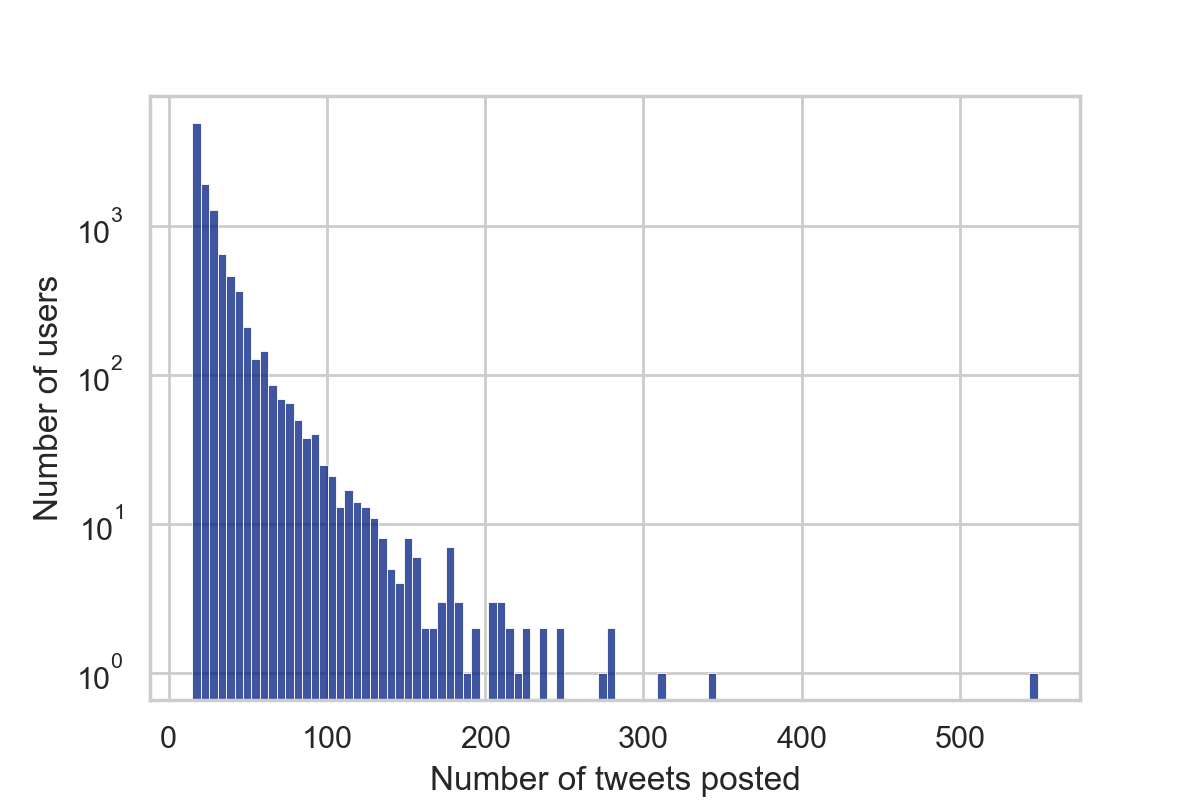
\includegraphics[width=0.5\textwidth]{user_per_tweet}
    \caption[Histogram of users per tweets]{Histogram representing the number of users per number of tweets}
    \label{fig:user_per_tweet}
\end{figure}
Analysing the user average sentiment distribution (figure \ref{fig:average_user_sentiment}), it is possible to notice that there are many users whose tweets are almost exclusively positive (or negative).
\begin{figure}
    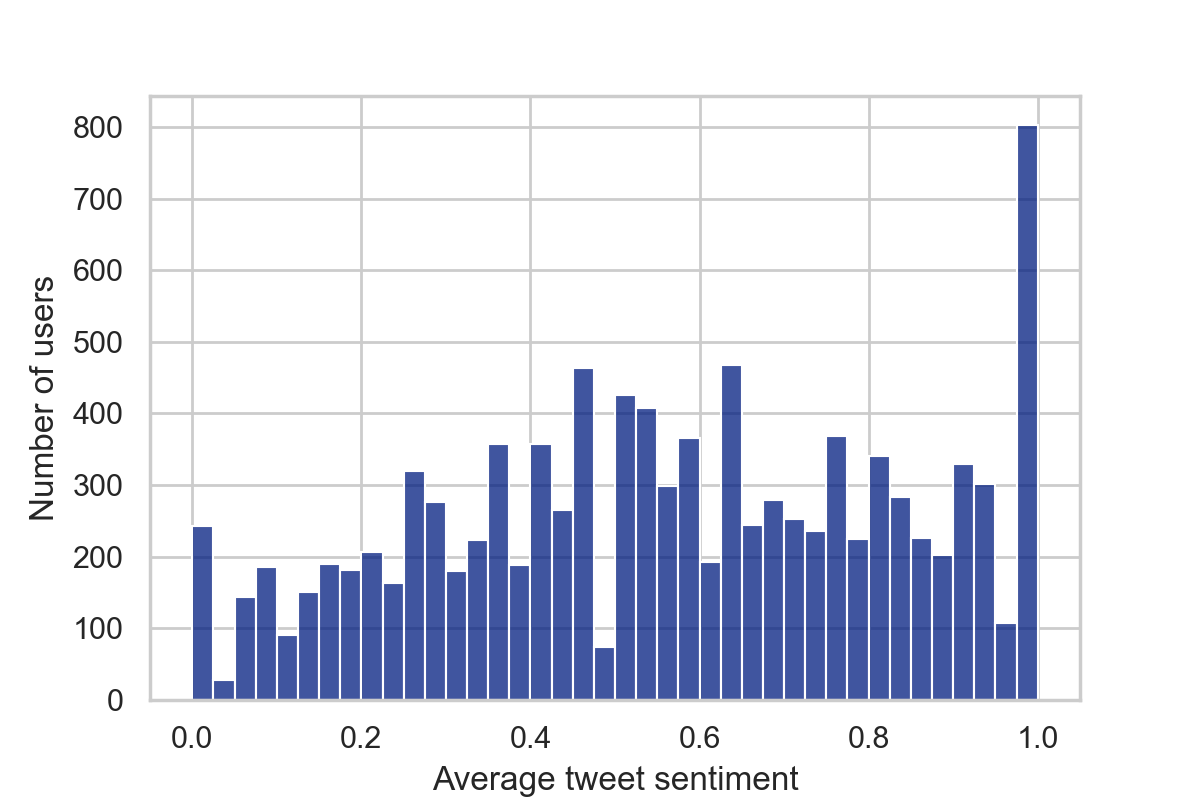
\includegraphics[width=0.5\textwidth]{average_user_sentiment}
    \caption[User average sentiment]{Histogram representing the number of users per average sentiment}
    \label{fig:average_user_sentiment}
\end{figure}
This odd behaviour led to a deeper investigation of the texts written by each user; a mean cosine similarity among the tweets posted by the same user was computed (figure \ref{fig:internal_similarity_users}), and it showed that a small but significant group of users used the exact same words in multiple tweets.  
\begin{figure}
    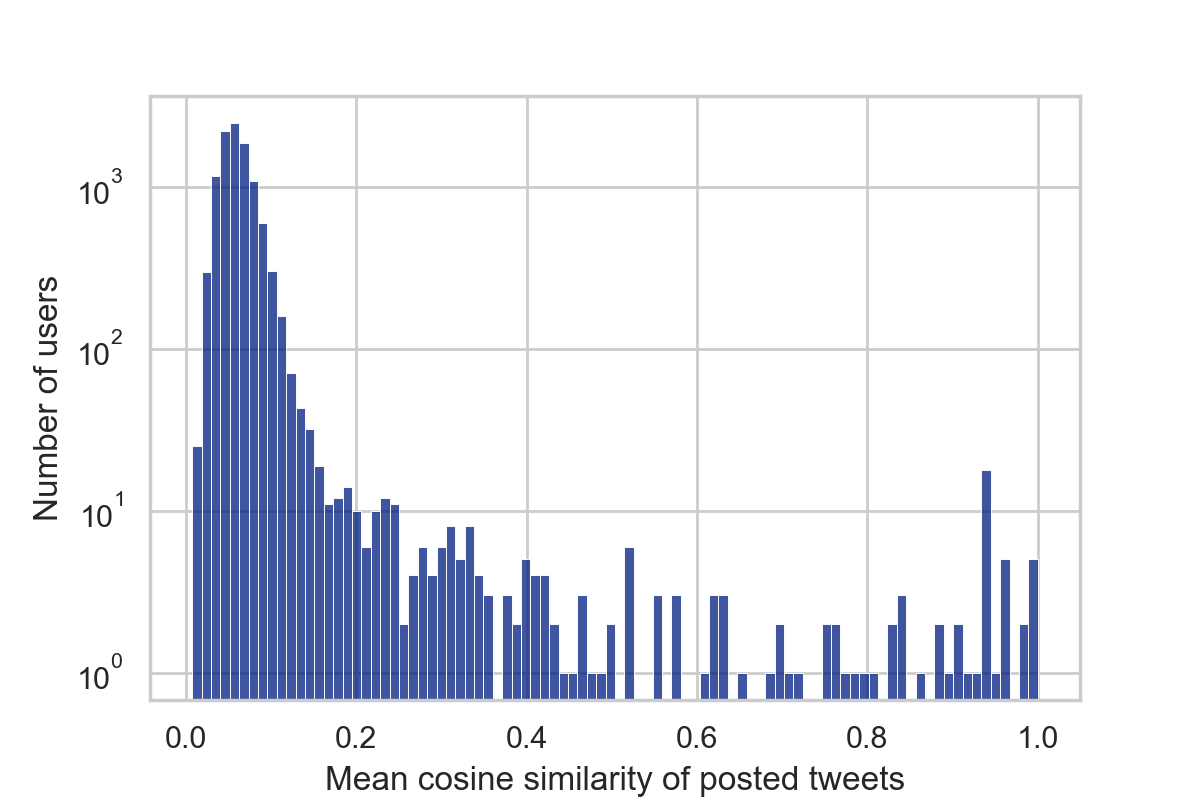
\includegraphics[width=0.5\textwidth]{internal_similarity_users}
    \caption[Mean cosine similarity]{Histogram representing the number of users per mean cosine similarity computed on the posted tweets of each user}
    \label{fig:internal_similarity_users}
\end{figure}
Some of the users that posted the largest number of tweets, also have the highest average cosine similarity among their tweets; a precise inspection of these users suggests that most of them behave as bots, regularly posting the same message. The problem of bot identification can be addressed using machine learning frameworks, as the one suggested by Kantepe and Ganiz \cite{8093483}. However, for this project a more naive approach to remove suspicious users is implemented in the preprocessing step. \\
Finally, the \textit{text} field collects the tweet messages. The messages are written in english, they may contain tags (i.e., words starting with "@"), hashtags (i.e., words starting with "\#"), and URLs. HTML character entities (e.g., "\textit{\&amp;}", "\textit{\&quot;}") are also present. \\
The \textit{text} field is the only one which is going to be considered to train the model and to predict the text sentiment; indeed, the \textit{date} field is only useful to show that both the development set and the evaluation set refer to the same time period; instead, the \textit{user} field is not taken into account because this would instruct the model to predict the sentiment considering also the user who posted the message, loosing the more general scope the model should have, that is to foresee the text sentiment regardless of the writer. 

\section{Proposed approach}
\subsection{Preprocessing}
The model evaluation is made using the evaluation set as reference. As said before, the development set and the evaluation set share the same characteristics, and, presumably, the same source. Basing the model performance on this evaluation set may lead to overfitting, making the model inadequate to predict the tweet sentiment outside this project. Therefore, two possible preprocessing paths have been designed: one more complex, composed of several steps, and more suitable to a general application; and one much simpler, consisting only of 3 steps, likely more context-dependent. The message cleaning steps composing the more articulate preprocessing path, partially influenced by Zainuddin et al. \cite{ZainuddinNurulhuda2016TFSa}, are the following
\begin{enumerate}
    \item Removal of rows having duplicate \textit{id} values;
    \item "\textit{\&amp;}" and "\textit{\&quot;}" HTML entities are removed; 
    \item Words starting with \textit{@} or \textit{http} are removed: these items are respectively user tags and URLs, and do not give insights regarding the sentiment of the message; 
    \item Removal of subsequent double letters: in any word, only one letter is kept if two or more consecutive letters are the same; this is useful to reduce to single word items that are written in different ways because the user wanted to imitate the colloquial language\footnote{For example, some users wrote "\textit{aw}" with a variable number of "\textit{w}"s at the end, but they were all expressing the same sentiment.};
    \item Punctuation is removed;
    \item Stemming is performed, using the Snowball stemmer designed by Porter \cite{Porter2006};
    \item Negations in sentences are stressed appending in subsequent words a "\textit{\_NEG}" suffix;
    \item Exclusion of users behaving as bots: as seen before, some users write the same message multiple times (i.e., users that have an high average cosine similarity computed on their tweets), and their message are almost always labelled with the same sentiment. These users should be excluded because they "pullute" the dataset, since the N-Grams\footnote{A N-Gram is a contiguous sequence of N items from a given sample of text or speech; if the items are words, N-Grams are also called \textit{shingles}.} contained in their sentences are going to be strongly associated by the model with the labelled sentiment of those messages. To identify the most damaging ones, for each user a \textit{user\_suspiciousness} metric was computed\footnote{The \textit{user\_suspiciousness} is computed as the product between the mean cosine similarity among the same user messages, and the "extremism" of their sentiment, that is the distance between the user message average sentiment and a neutral sentiment (i.e., 0.5); both the mean cosine similarity and the sentiment extremism are scaled between 0 and 1 before the product.}, and the users having a value higher than 0.9 were dropped from the development set;
    \item Conversion of all the characters to lowercase.
\end{enumerate}
After these steps, the features are extracted tokenizing the messages and creating a bag-of-words; the schema applied to weight the words is the \textbf{tf-idf} (\textit{term frequency - inverse document frequency}), meaning that each word importance increases as its frequency in the same meassage increases, and lowers the more the word is used across all messages in the collection. No maximum or minimum document frequency is set for a word to be considered. Other preprocessing options, such as the removal of stopwords, the type of normalization, and the N-Gram length, are treated as hyperparameters of the preprocessing step and tuned using a grid search in conjunction with the model hyperparameters.\\
Concerning the shorter preprocessing path, it only includes steps 1, 2, 9 of the longer path, and also the word tokenization with tf-idf weights. This preprocessing option has not been taken into account during in the model tuning operations, but its usage is briefly discussed at the end of the Results paragraph. 
\subsection{Model selection}
Two fast and light classification models have been chosen for evaluation: 
\begin{itemize}
    \item Naive Bayes Classifier: it is a classifier family commonly employed in sentiment analysis contexts \cite{MEDHAT20141093}. It uses the Bayes Theorem to predict the probability that a given feature set belongs to a particular label. The Naive Bayes Classifier family include several algorithms, in particular the Multinomial and the Bernoulli classifiers are often applied in textual document classification, with similar performance \cite{8776800}. For this project, given that the tf-idf word weighting schema is used instead of a basic term occurrence, the Multinomial Naive Bayes Classifier (\textbf{Multinomial NB}) was selected.
    \item Support Vector Machine Classifier: these algorithms carry out the classification task determining the separators in the search space which can best separate the different classes. SVCs have already been used in sentiment analysis contexts, achieving good results \cite{6914200}. Because of the extent of the dataset, in particular concerning the features, only the simpler Linear Support Vector Classifier (\textbf{Linear SVC}) was considered. 
\end{itemize}
The best performing hyperparameter configuration was identified using a grid search. 
\subsection{Hyperparameters tuning}
Both the preprocessing and the model hyperparameters were tuned. The considered hyperparameter configurations are summarized in table \ref{table: hyperparameters_considered}.
\begin{table}[]
    \caption{Considered hyperparameters}
    \begin{tabular}{l|c|c}
    \textbf{Preprocessing / Model} & \textbf{Hyperparameter}                                                                                                                                         & \textbf{Values}                                                                                                                                                                                             \\ \hline
    TfidfVectorizer                & \textit{\begin{tabular}[c]{@{}c@{}}stopwords\\ ngram\_range\\ max\_features\\ max\_df\\ min\_df\\ binary\\ norm\\ use\_idf\\ smooth\_idf\\ sublinear\_tf\end{tabular}} & \begin{tabular}[c]{@{}c@{}}\{"english",None\}\\ \{(1,1),(1,2),(1,3)\}\\ \{None,20000\}\\ \{1.0\}\\ \{1\}\\ \{True,False\}\\ \{l1,l2\}\\ \{True\}\\ \{True,False\}\\ \{False\}\end{tabular} \\ \hline
    Multinomial NB                 & \textit{alpha}                                                                                                                                                  & \{.01,.02,.05,.1,.2,.5,1.0\}                                                                                                                                                                    \\ \hline
    SVC                            & \textit{\begin{tabular}[c]{@{}c@{}}penalty\\ tolerance\\ C\\ max\_iter\end{tabular}}                                                                       & \begin{tabular}[c]{@{}c@{}}\{l1,l2\}\\ \{1e-2,1e-3\}\\ \{1,10\}\\ \{100\}\end{tabular}                                                                                                              
    \end{tabular}
	\label{table: hyperparameters_considered}
\end{table}
The development set is 90/10 train/validation splitted, given that the development set is fairly large, and a grid search is run on the traning subset. 
\section{Results}
The best configuration found for the preprocessing step is almost the same using the Linear SVC and the Multinomial NB, differentiating by only one parameter:
\begin{itemize}
    \item \textit{stopwords}: None 
    \item \textit{ngram\_range}: (1,3)
    \item \textit{max\_features}: None
    \item \textit{binary}: True
    \item \textit{norm}: l2
    \item \textit{smooth\_idf}: False for the Linear SVC, True for the Multinomial NB
\end{itemize}
Notably, for both models, the grid search suggested that no words should be removed, neither using stopwords nor setting an upper limit for the feature number; this seems reasonable given the context of the project. Indeed, when analysing a message sentiment, dropping some words can make unclear and ambiguous the meaning of the text, reducing the algorithm classification capability.\\
Concerning the model tuning, the best configurations found, and the respective reached \textit{f1 macro scores}, are the following:
\begin{itemize}
    \item Linear SVC: best $f1\:macro \approx 0.794$
    \begin{itemize}
        \item \textit{penalty}: l2
        \item \textit{tolerance}: 0.001
        \item \textit{C}: 1
    \end{itemize}
    \item Multinomial NB: best $f1\:macro \approx 0.758$
    \begin{itemize}
        \item \textit{alpha}: 0.1
    \end{itemize}
\end{itemize}
After training the best performing Linear SVC and Multinomial NB on all available development data, and using these models to predict the labels in the evaluation set, the obtained public f1 scores are respectively 0.802 and 0.764. \\
\begin{figure}
    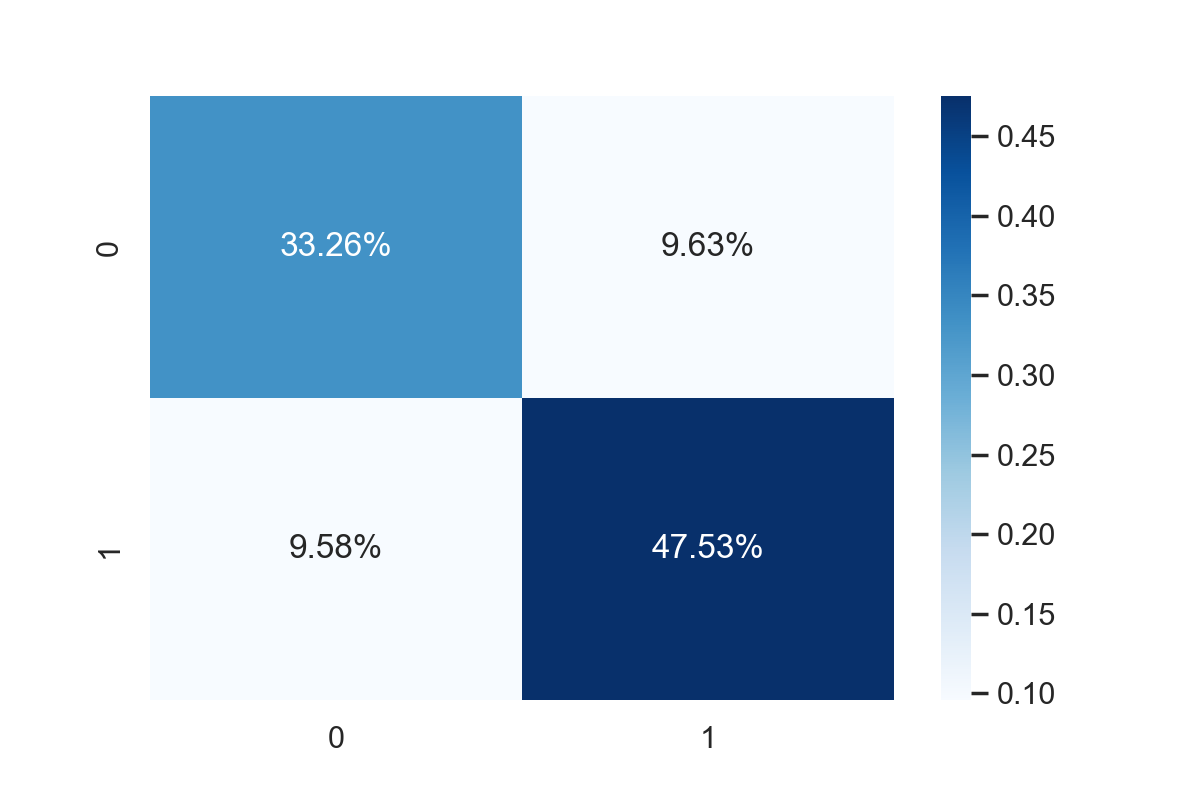
\includegraphics[width=0.5\textwidth]{conf_matrix_SVC}
    \caption[Linear SVC confusion matrix]{Confusion matrix of the results obtained using the Linear SVC model}
    \label{fig:conf_matrix_SVC}
\end{figure}
\begin{figure}
    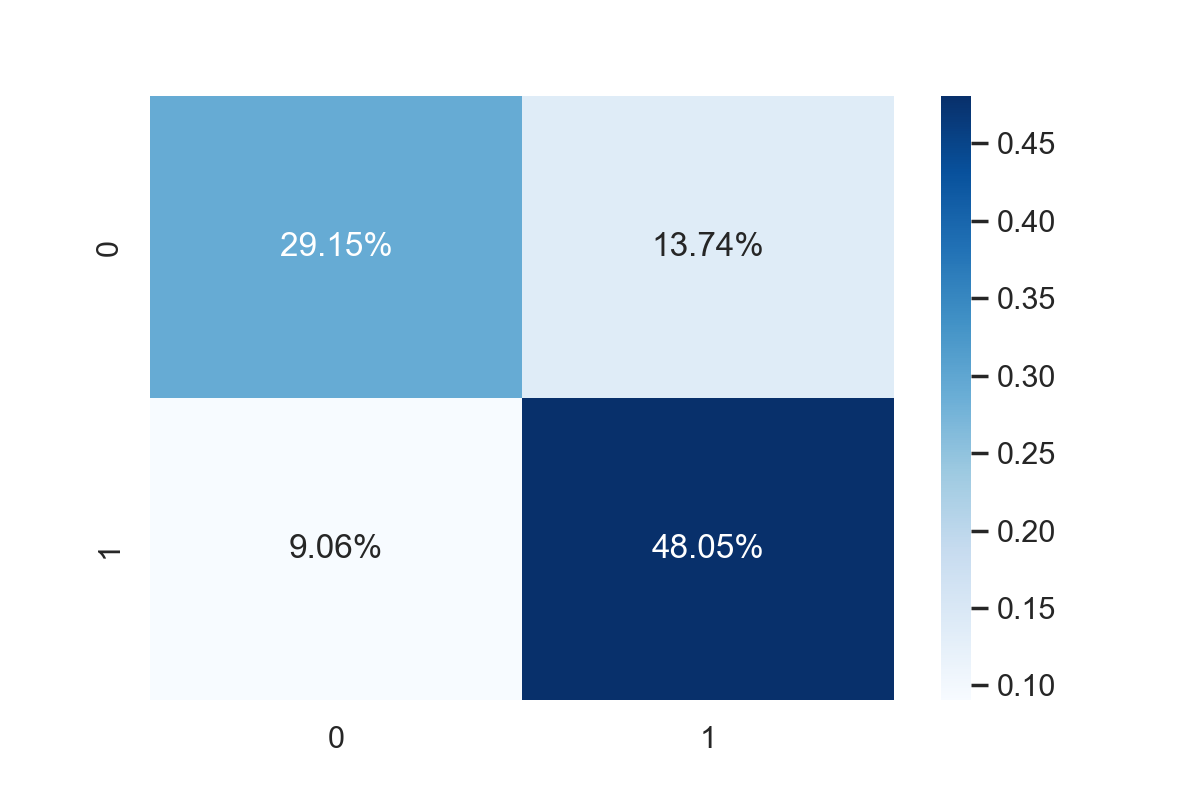
\includegraphics[width=0.5\textwidth]{conf_matrix_NB}
    \caption[Multinomial NB confusion matrix]{Confusion matrix of the results obtained using the Multinomial NB model}
    \label{fig:conf_matrix_NB}
\end{figure}
So, it is possible to conclude that the Linear SVC model achieves better results than the Multinomial NB model. The confusion matrices in figures \ref{fig:conf_matrix_SVC} and \ref{fig:conf_matrix_NB} give an insight of where the Linear SVC outperforms the Multinomial NB model: even if the latter one is slightly better in predicting the positive sentiment, it is much worse when it comes to messages with negative sentiment. This may be due to the fact that the Linear SVC model is more capable to deal with the label unbalance afflicting the development set. \\
\begin{figure}
    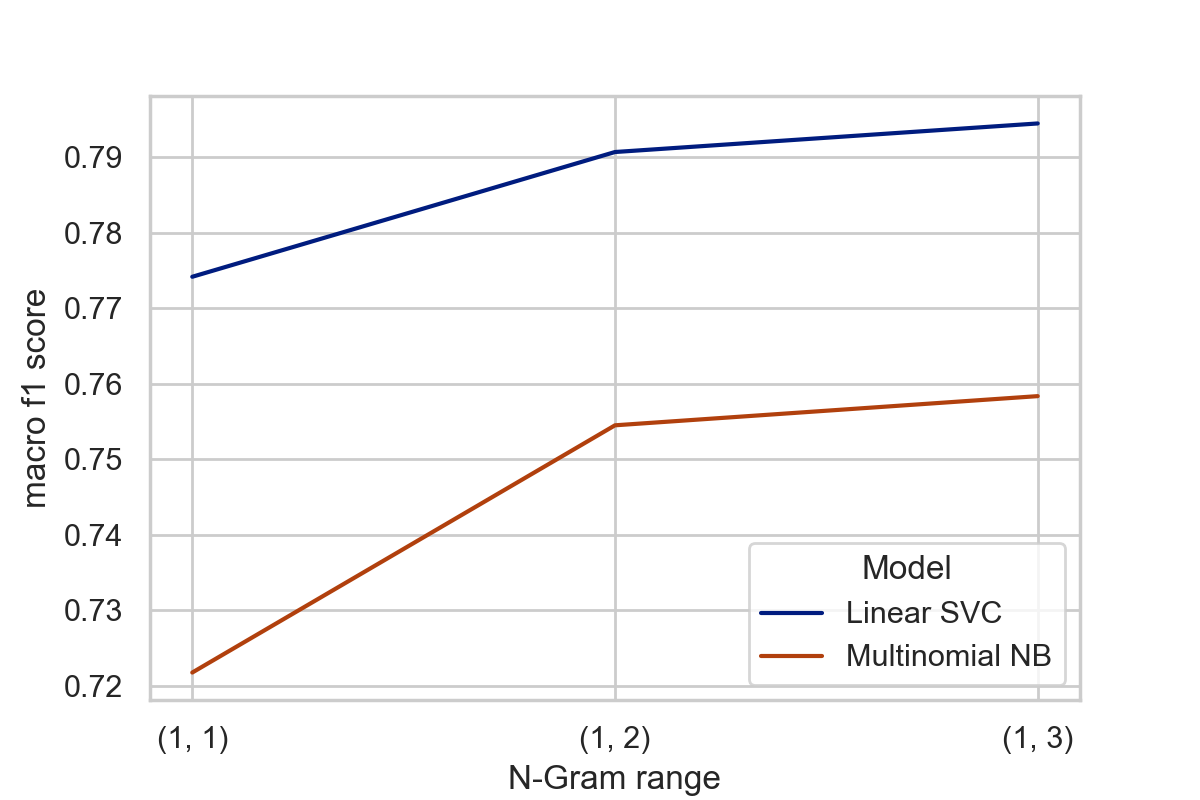
\includegraphics[width=0.5\textwidth]{ngram_f1_score}
    \caption[F1 score as function of N-Gram range]{Performance of f1 score for different N-gram lengths}
    \label{fig:ngram_f1_score}
\end{figure}
To conclude, it is interesting to see how much the results are influenced by the N-Gram range parameter. This parameter controls the length of the N-Grams to consider during the word tokenization, so $ngram\_range=(1,1)$ means that only single words are considered, while $ngram\_range=(1,3)$ means that also bigrams and trigrams are included in the bag-of-words. As figure \ref{fig:ngram_f1_score} shows, increasing the N-Gram length considerably improves the model results: this trend suggests the importance of word combinations to express a sentiment, and also, conversely, to understand the sentiment embedded in a sentence.\\
For the sake of completeness, the tuned Linear SVC model has also been tested using the shorter preprocessing path, and it reached a public f1 score equal to 0.805. So, this preprocessing path seems to lead to better results than the more complex one, but it is due to the similarity of the evaluation set with the development set; therefore, in the limited scope of this project, it performs better, but it would probably not perform as well in a more generic application.

\section{Discussion}
Both the solutions found using the tuned models overcome the baseline score of 0.753. In particular, the Linear Support Vector Classifier reaches good results, especially considering the model simplicity and speed. However, the critical step in this project was the document preprocessing: the usage of bigrams and trigrams combined with unigrams led to a wide increase in the f1-score.\\
Many hyperparameter configurations were left unexplored, and maybe, using a more granular grid search, it is still possible to improve the results. However, to really further enhance the obtained score, other more complex machine learning models should be considered, such as non linear SVCs or ANNs, maybe preceded by the application of a dimensionality reduction algorithm, like SVD, to reduce the number of features and to extract the most meaningful ones. \\Another possible solution to explore is the usage of deep learning models with a word embedding layer, that could also be based on a pretrained word embedding stack, substantially reducing the time required for the model training. The use of deep learning models in the context of sentiment analysis has been widely tackled in recent years, with good results (see Zhang et al. \cite{ZhangLeiWangShuaiLiuBing}). \\It might also be interesting to apply an unsupervised machine learning method to the dataset and compare its results with the supervised methods. To this end, a promising candidate model is VADER, that was designed specifically for sentiment analysis, and is sensitive to both polarity (positive/negative) and intensity (strength) of emotions expressed in texts; the usage of this model in a context analogous to the one of this project is discussed by Elbagir and Yang \cite{elbagir2019twitter}.

\bibliography{bibliography}
\bibliographystyle{ieeetr}

\end{document}
